\chapter{Markov Blankets}


This chapter is based on the
Wikipedia article, 
Ref.\cite{wiki-mblanket}.
Markov blankets
and Markov boundaries of bnets
were apparently invented
by Judea Pearl. His 1988 book
 Ref.\cite{Pearl-mblanket}, 
instead of a research paper, is 
usually given as the original reference.

\begin{figure}[h!]
\centering
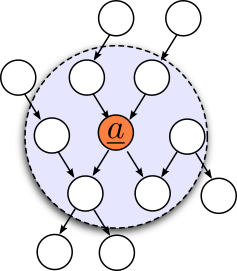
\includegraphics[width=3in]{mblanket/mblanket.png}
\caption{In a bnet,
the minimal Markov blanket,
aka Markov boundary,
of node $\rva$.} 
\label{fig-mblanket}
\end{figure}

We will treat vectors 
of random variables as if
they were sets when using the $\in$,
$\subset$ and $-$ operations.
For example,
if $\rvx=(\rvx_0, 
\rvx_1, \rvx_2,
\rvx_3)$ and
$\rvb=(\rvx_1, \rvx_2)$,
then $\rvx_1\in \rvb\subset \rvx$ and
$\rvx-\rvb=(\rvx_0, \rvx_3)$.

Below, $D(\rva:\rvb|\rvc)$
denotes the conditional
mutual information of
random variables
$\rva$ and $\rvb$
conditioned on 
random variable $\rvc$.
$D(\rva:\rvb|\rvc)=0$
iff $\rva$ and $\rvb$
are independent
when $\rvc$ is held fixed.
$D(\rva:\rvb|\rvc)$
is used in Shannon Information
Theory.


Suppose
$\rva\in  \rvX$,
 $\rvB\subset \rvX$,
but $\rva\notin\rvB$.
Then $\rvB$ is a Markov blanket
of $\rva$ if

\beq
D(\rva: \rvX-\rva|\rvB)=0
\;.
\eeq

The minimal Markov blanket 
is called the Markov boundary.

In a bnet, the minimal Markov blanket,
aka Markov boundary,
of a node $\rva$,
includes:
\begin{enumerate}
\item
parents of $\rva$
\item
children of $\rva$
\item
parents of childern of $\rva$
\end{enumerate}
This is illustrated in 
Fig.\ref{fig-mblanket}.